\textbf{COLUNI 2026 -- Questão 19}\par\medskip No gráfico abaixo são apresentados alguns resultados de uma pesquisa a respeito do preço de um pente de ovos contendo 30 unidades, no período de outubro de 2024 a junho de 2025.

% COLUNI-AUTO-FIGURES-BEGIN
\begin{figure}[htbp]
\centering
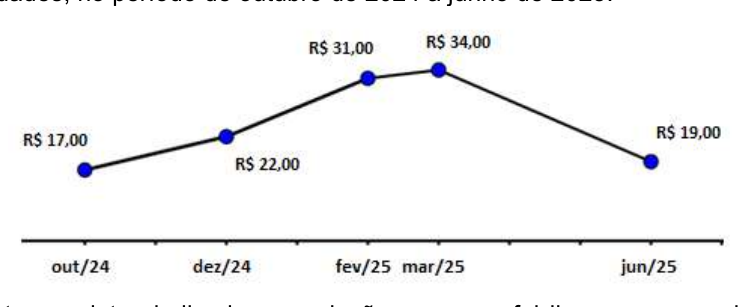
\includegraphics[width=0.75\linewidth]{static/simulados/coluni/figuras/2026/questao-19/figura-1.png}
\end{figure}
% COLUNI-AUTO-FIGURES-END

Considerando que entre as datas indicadas a variação no preço foi linear e que cada marcação no eixo horizontal indicava os meses em que ocorreu a pesquisa, é CORRETO afirmar que:
\begin{enumerate}
\item Por sete meses o preço do pente de ovos foi maior que R\$20,00.
\item O preço do pente de ovos nos meses de dez/24 e mai/25 foi o mesmo.
\item No mês de abr/25 o preço de um ovo retirado desse pente era menor que R\$1,00.
\item A média aritmética do preço do pente de ovos entre out/24 e jun/25 é R\$26,00.
\end{enumerate}
